% questions.tex —— 2008 年·普通高等学校招生考试·湖南卷·理科 · 题目内容片段（无答案）
% 由 tools/generate_projects.py 依来源总账自 2008/2008_数学真题_湖南理_试题.md 生成，勿手改（改源 MD 后重跑）


\gkpart{一、选择题}

\begin{question}
\gkti{1}复数 $\left(\mathrm i-\dfrac1{\mathrm i}\right)^3$ 等于（　）

（A）$8$

（B）$-8$

（C）$8\mathrm i$

（D）$-8\mathrm i$

\end{question}
\begin{question}
\gkti{2}“$|x-1|<2$ 成立”是“$x(x-3)<0$ 成立”的（　）

（A）充分不必要条件

（B）必要不充分条件

（C）充分必要条件

（D）既不充分也不必要条件

\end{question}
\begin{question}
\gkti{3}已知变量 $x$，$y$ 满足条件 $\begin{cases}x\geqslant1,\\ x-y\leqslant0,\\ x+2y-9\leqslant0,\end{cases}$ 则 $x+y$ 的最大值是（　）

（A）$2$

（B）$5$

（C）$6$

（D）$8$

\end{question}
\begin{question}
\gkti{4}设随机变量 $\xi$ 服从正态分布 $N(2,9)$，若 $P(\xi>c+1)=P(\xi<c-1)$，则 $c=$（　）

（A）$1$

（B）$2$

（C）$3$

（D）$4$

\end{question}
\begin{question}
\gkti{5}设有直线 $m$、$n$ 和平面 $\alpha$、$\beta$。下列四个命题中，正确的是（　）

（A）若 $m\parallel\alpha$，$n\parallel\alpha$，则 $m\parallel n$

（B）若 $m\subset\alpha$，$n\subset\alpha$，$m\parallel\beta$，$n\parallel\beta$，则 $\alpha\parallel\beta$

（C）若 $\alpha\perp\beta$，$m\subset\alpha$，则 $m\perp\beta$

（D）若 $\alpha\perp\beta$，$m\perp\beta$，$m\not\subset\alpha$，则 $m\parallel\alpha$

\end{question}
\begin{question}
\gkti{6}函数 $f(x)=\sin^2x+\sqrt3\sin x\cos x$ 在区间 $\left[\dfrac\pi4,\dfrac\pi2\right]$ 上的最大值是（　）

（A）$1$

（B）$\dfrac{1+\sqrt3}2$

（C）$\dfrac32$

（D）$1+\sqrt3$

\end{question}
\begin{question}
\gkti{7}设 $D$、$E$、$F$ 分别是 $\triangle ABC$ 的三边 $BC$、$CA$、$AB$ 上的点，且 $\overrightarrow{DC}=2\overrightarrow{BD}$，$\overrightarrow{CE}=2\overrightarrow{EA}$，$\overrightarrow{AF}=2\overrightarrow{FB}$，则 $\overrightarrow{AD}+\overrightarrow{BE}+\overrightarrow{CF}$ 与 $\overrightarrow{BC}$（　）

（A）反向平行

（B）同向平行

（C）互相垂直

（D）既不平行也不垂直

\end{question}
\begin{question}
\gkti{8}若双曲线 $\dfrac{x^2}{a^2}-\dfrac{y^2}{b^2}=1$（$a>0$，$b>0$）上横坐标为 $\dfrac{3a}2$ 的点到右焦点的距离大于它到左准线的距离，则双曲线离心率的取值范围是（　）

（A）$(1,2)$

（B）$(2,+\infty)$

（C）$(1,5)$

（D）$(5,+\infty)$

\end{question}
\begin{question}
\gkti{9}长方体 $ABCD-A_1B_1C_1D_1$ 的 $8$ 个顶点在同一个球面上，且 $AB=2$，$AD=\sqrt3$，$AA_1=1$，则顶点 $A$、$B$ 间的球面距离是（　）

（A）$2\sqrt2\pi$

（B）$\sqrt2\pi$

（C）$\dfrac{\sqrt2\pi}2$

（D）$\dfrac{\sqrt2\pi}4$

\end{question}
\begin{question}
\gkti{10}设 $[x]$ 表示不超过 $x$ 的最大整数（如 $[2]=2$，$\left[\dfrac54\right]=1$）。对于给定的 $n\in\mathbf N^*$，定义 $\mathrm C_n^x=\dfrac{n(n-1)\cdots(n-[x]+1)}{x(x-1)\cdots(x-[x]+1)}$，$x\in[1,+\infty)$，则当 $x\in\left[\dfrac32,3\right)$ 时，函数 $\mathrm C_8^x$ 的值域是（　）

（A）$\left[\dfrac{16}3,28\right]$

（B）$\left[\dfrac{16}3,56\right)$

（C）$\left(4,\dfrac{28}3\right)\cup[28,56)$

（D）$\left(4,\dfrac{16}3\right]\cup\left(\dfrac{28}3,28\right]$

\end{question}
\gkpart{二、填空题}

\begin{question}
\gkti{11}$\lim\limits_{x\to1}\dfrac{x-1}{x^2+3x-4}=$\gkblank{}。

\end{question}
\begin{question}
\gkti{12}已知椭圆 $\dfrac{x^2}{a^2}+\dfrac{y^2}{b^2}=1$（$a>b>0$）的右焦点为 $F$，右准线为 $l$，离心率 $e=\dfrac{\sqrt5}5$。过顶点 $A(0,b)$ 作 $AM\perp l$，垂足为 $M$，则直线 $FM$ 的斜率等于\gkblank{}。

\end{question}
\begin{question}
\gkti{13}设函数 $y=f(x)$ 存在反函数 $y=f^{-1}(x)$，且函数 $y=x-f(x)$ 的图象过点 $(1,2)$，则函数 $y=f^{-1}(x)-x$ 的图象一定过点\gkblank{}。

\end{question}
\begin{question}
\gkti{14}已知函数 $f(x)=\dfrac{\sqrt{3-ax}}{a-1}$（$a\neq1$）。

（1）若 $a>1$，则 $f(x)$ 的定义域是\gkblank{}；

（2）若 $f(x)$ 在区间 $(0,1]$ 上是减函数，则实数 $a$ 的取值范围是\gkblank{}。

\end{question}
\begin{question}
\gkti{15}对有 $n$（$n\geqslant4$）个元素的总体 $\{1,2,3,\cdots,n\}$ 进行抽样，先将总体分成两个子总体 $\{1,2,\cdots,m\}$ 和 $\{m+1,m+2,\cdots,n\}$（$m$ 是给定的正整数，且 $2\leqslant m\leqslant n-2$），再从每个子总体中各随机抽取 $2$ 个元素组成样本，用 $P_{ij}$ 表示元素 $i$ 和 $j$ 同时出现在样本中的概率，则 $P_{1n}=$\gkblank{}；所有 $P_{ij}$（$1\leqslant i<j\leqslant n$）的和等于\gkblank{}。

\end{question}
\gkpart{三、解答题}

\begin{question}
\gkti{16}甲、乙、丙三人参加了一家公司的招聘面试，面试合格者可正式签约。甲表示只要面试合格就签约。乙、丙则约定：两人面试都合格就一同签约，否则两人都不签约。设每人面试合格的概率都是 $\dfrac12$，且面试是否合格互不影响。求：

（1）至少有 $1$ 人面试合格的概率；

（2）签约人数 $\xi$ 的分布列和数学期望。

\Needspace{0.4\textheight}
\end{question}
\begin{question}
\gkti{17}如图所示，四棱锥 $P-ABCD$ 的底面 $ABCD$ 是边长为 $1$ 的菱形，$\angle BCD=60^\circ$，$E$ 是 $CD$ 的中点，$PA\perp$ 底面 $ABCD$，$PA=2$。

（1）证明：平面 $PBE\perp$ 平面 $PAB$；

（2）求平面 $PAD$ 和平面 $PBE$ 所成二面角（锐角）的大小。
\nopagebreak[4]
\begin{center}% 2008 年湖南卷理科第 17 题：四棱锥 P-ABCD，底面 ABCD 是边长 1 的菱形，∠BCD=60°，
%   E 是 CD 的中点，PA ⊥ 底面，PA=2。
% 来源 PDF：gaokaomath-src/普通高考/2008/2008湖南理.pdf
% SHA-256：a702a9a7fbdfa2d31961e21e2da7a555ce4ad67771f88fa28c9f99d659b913d7
% 原页：2008湖南理.pdf 第 1 页（A3 三栏）第 3 栏，书页码 453。
% 绘制依据：底面取斜投影 (x,y)->(x+0.5y, 0.55y)，正三角形 ABD 与 BCD 共边；
%   A(0,0)、B(1,0)、D(0.5,0.866)、C(1.5,0.866)，P 在 A 的正上方（高 2），E 为 CD 中点。
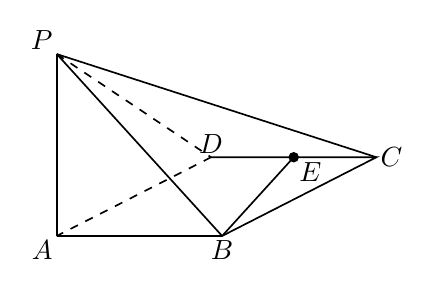
\begin{tikzpicture}[scale=2.1, semithick, every node/.style={inner sep=1.2pt}]
  \coordinate (A) at (0.00,0.00);
  \coordinate (B) at (1.00,0.00);
  \coordinate (D) at (0.933,0.476);
  \coordinate (C) at (1.933,0.476);
  \coordinate (P) at (0.00,1.10);
  \coordinate (E) at (1.433,0.476);

  % 底面
  \draw (A) -- (B) -- (C) -- (D);
  \draw[dashed] (D) -- (A);

  % 侧棱
  \draw (P) -- (A);
  \draw (P) -- (B);
  \draw (P) -- (C);
  \draw[dashed] (P) -- (D);

  % BE
  \draw (B) -- (E);

  \fill (E) circle (0.9pt);

  \node[below left] at (A) {$A$};
  \node[below] at (B) {$B$};
  \node[right] at (C) {$C$};
  \node[above] at (D) {$D$};
  \node[above left] at (P) {$P$};
  \node[below right=0.5pt] at (E) {$E$};
\end{tikzpicture}
\end{center}
\nopagebreak[4]
\end{question}
\begin{question}
\gkti{18}数列 $\{a_n\}$ 满足 $a_1=1$，$a_2=2$，$a_{n+2}=\left(1+\cos^2\dfrac{n\pi}2\right)a_n+\sin^2\dfrac{n\pi}2$，$n=1,2,3,\cdots$。

（1）求 $a_3$，$a_4$，并求数列 $\{a_n\}$ 的通项公式；

（2）设 $b_n=\dfrac{a_{2n-1}}{a_{2n}}$，$S_n=b_1+b_2+\cdots+b_n$。证明：当 $n\geqslant6$ 时，$|S_n-2|<\dfrac1n$。

\end{question}
\begin{question}
\gkti{19}在一个特定时段内，以点 $E$ 为中心的 $7$ 海里以内海域被设为警戒水域。点 $E$ 正北 $55$ 海里处有一个雷达观测站 $A$。某时刻测得一艘匀速直线行驶的船只位于点 $A$ 北偏东 $45^\circ$ 且与点 $A$ 相距 $40\sqrt2$ 海里的位置 $B$，经过 $40$ 分钟又测得该船已行驶到点 $A$ 北偏东 $45^\circ+\theta$（其中 $\sin\theta=\dfrac{\sqrt{26}}{26}$，$0^\circ<\theta<90^\circ$）且与点 $A$ 相距 $10\sqrt{13}$ 海里的位置 $C$。

（1）求该船的行驶速度（单位：海里/小时）；

（2）若该船不改变航行方向继续行驶，判断它是否会进入警戒水域，并说明理由。

\end{question}
\begin{question}
\gkti{20}若 $A$、$B$ 是抛物线 $y^2=4x$ 上的不同两点，弦 $AB$（不平行于 $y$ 轴）的垂直平分线与 $x$ 轴相交于点 $P$，则称弦 $AB$ 是点 $P$ 的一条“相关弦”。已知当 $x>2$ 时，点 $P(x,0)$ 存在无穷多条“相关弦”。给定 $x_0>2$。

（1）证明：点 $P(x_0,0)$ 的所有“相关弦”的中点的横坐标相同；

（2）试问：点 $P(x_0,0)$ 的“相关弦”的弦长中是否存在最大值？若存在，求其最大值（用 $x_0$ 表示）；若不存在，请说明理由。

\end{question}
\begin{question}
\gkti{21}已知函数 $f(x)=\ln^2(1+x)-\dfrac{x^2}{1+x}$。

（1）求函数 $f(x)$ 的单调区间；

（2）若不等式 $\left(1+\dfrac1n\right)^{n+\alpha}\leqslant\mathrm e$ 对任意的 $n\in\mathbf N^*$ 都成立（其中 $\mathrm e$ 是自然对数的底数），求 $\alpha$ 的最大值。

\end{question}